%&LaTeX
% !TEX encoding = UTF-8 Unicode
\documentclass{article}
\usepackage[utf8]{inputenc}
\usepackage[francais]{babel}
\usepackage[T1]{fontenc}
\usepackage{textcomp}
\usepackage[colorlinks=true, linkcolor=black, urlcolor = blue]{hyperref}

\usepackage{graphicx}
\usepackage{ulem}
\usepackage{color}
\usepackage[top=2.5cm,bottom=3cm,left=3cm,right=3cm]{geometry}

\definecolor{color01}{rgb}{0.00,0.00,0.00}
\definecolor{color02}{rgb}{0.40,0.40,0.40}
\definecolor{color04}{rgb}{0.07,0.33,0.80}
\definecolor{color05}{rgb}{1.00,0.00,0.00}


\title{\Huge{AGETAC\\
Aide à la GEstion TACtique\\}
\huge{{\color{color02} \textit{Manuel d'utilisation}}}}

\date{Mai 2012}
\author{Projet Agetac - Université de Rennes 1\\
Encadré par Noël Plouzeau}



\begin{document}
\maketitle
\vspace{1in}
\tableofcontents
\newpage
 \section{Objectifs}

L’intérêt de l’application est de faciliter la gestion d’une intervention pour les pompiers grâce a l’utilisation de tablettes tactiles pourvus de l’application Agetac. Les tablettes inter-connectées grâce a un serveur apporteront plus de rapidité et de précision, améliorant ainsi le bon déroulement d’une intervention.

\section{Création d’une intervention}

Une interface simple de création/consultation d’intervention est disponible.

Pour créer une intervention, entrez un nom d’intervention et les coordonnées GPS dans les champs prévus a cet effet.

\begin{figure}[h!]
\begin{center}
\includegraphics[width=7cm]{creationinter.png}
\caption{Création d'une intervention}
\end{center}
\end{figure}

\section{Utilisation de la tablette}

Assurez-vous toujours que la tablette dispose de suffisamment de batterie. Celle-ci doit pouvoir rester en marche pendant toute la durée d’une intervention. Il est possible de les recharger sur l’allume-cigare d’un véhicule avec un câble adapté.

\subsection{Connexion à une intervention}

Avant de vous rendre sur les lieux du sinistre, ou une fois sur place, mettez la tablette sous tension et identifiez-vous.

Une fois la connexion établie, l’onglet SITAC apparaît à l’écran. Il s’agit de l’onglet d’accueil.

Vous pouvez ensuite naviguer entre les différents onglets d’une simple pression sur ceux-ci.

\newpage
\subsection{Présentation des différents onglets}

\subsubsection{Onglet SITAC}

Cet onglet permet de visualiser l’intervention.

Il est composé d’une carte et d’un menu d’outils sur la gauche. Celui-ci permet de représenter la situation grâce aux différents pictogrammes regroupés par catégories.
\vspace{1.2in}
\begin{figure}[hbt]
\begin{center}
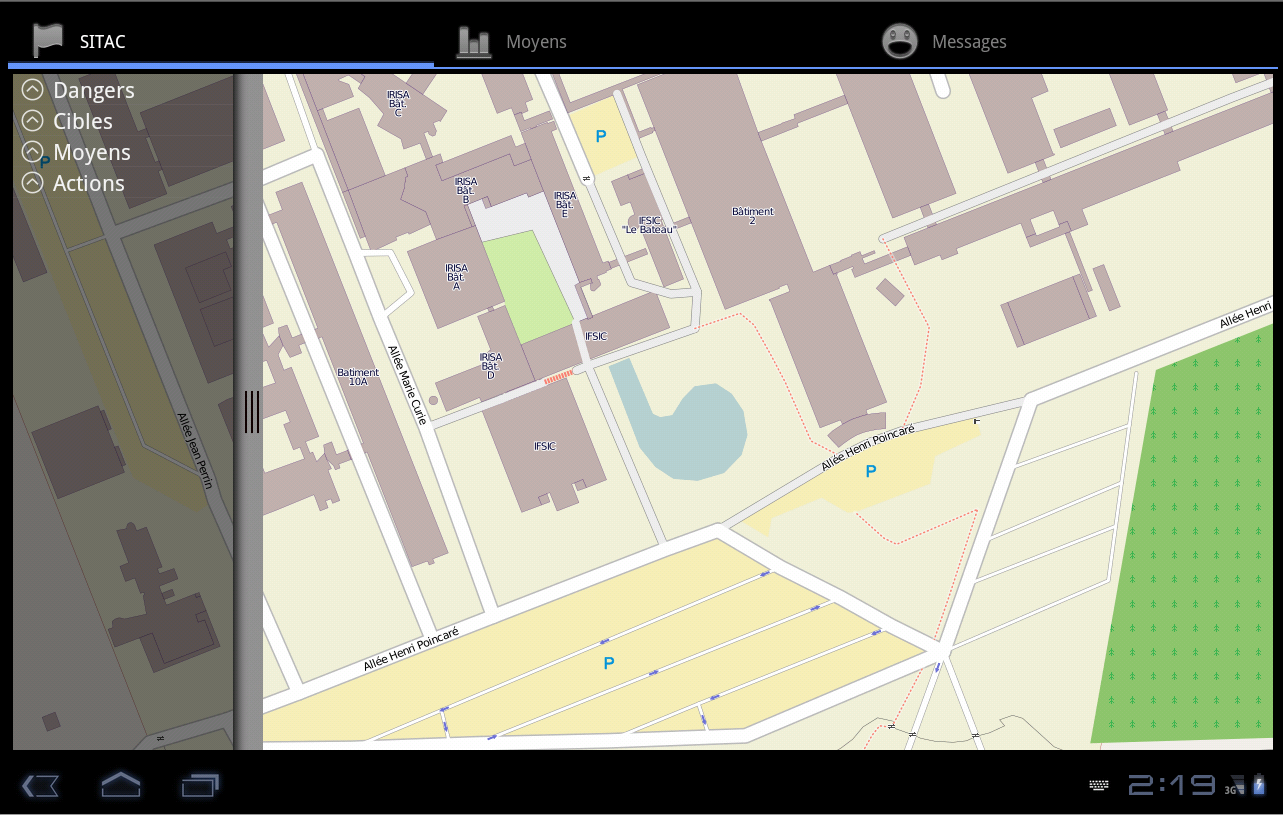
\includegraphics[width=470pt]{Manueldutilisation-fig001.png}
\caption{Vue de la SITAC}
\end{center}
\end{figure}

\newpage
\subsubsection{Onglet Moyens}

Cet onglet référence les moyens demandés et présents sur les lieux. Il permet de faire des demandes qui seront automatiquement transmises au CODIS, ou de renvoyer un véhicule si sa présence n’est plus nécessaire à l’intervention. Vous pouvez aussi y consulter tout ce qui est relatif à chaque véhicule (sa caserne d’origine, son groupe horaire de demande, d’arrivée et de départ)

\vspace{1.1in}

\begin{figure}[hbt]
\begin{center}
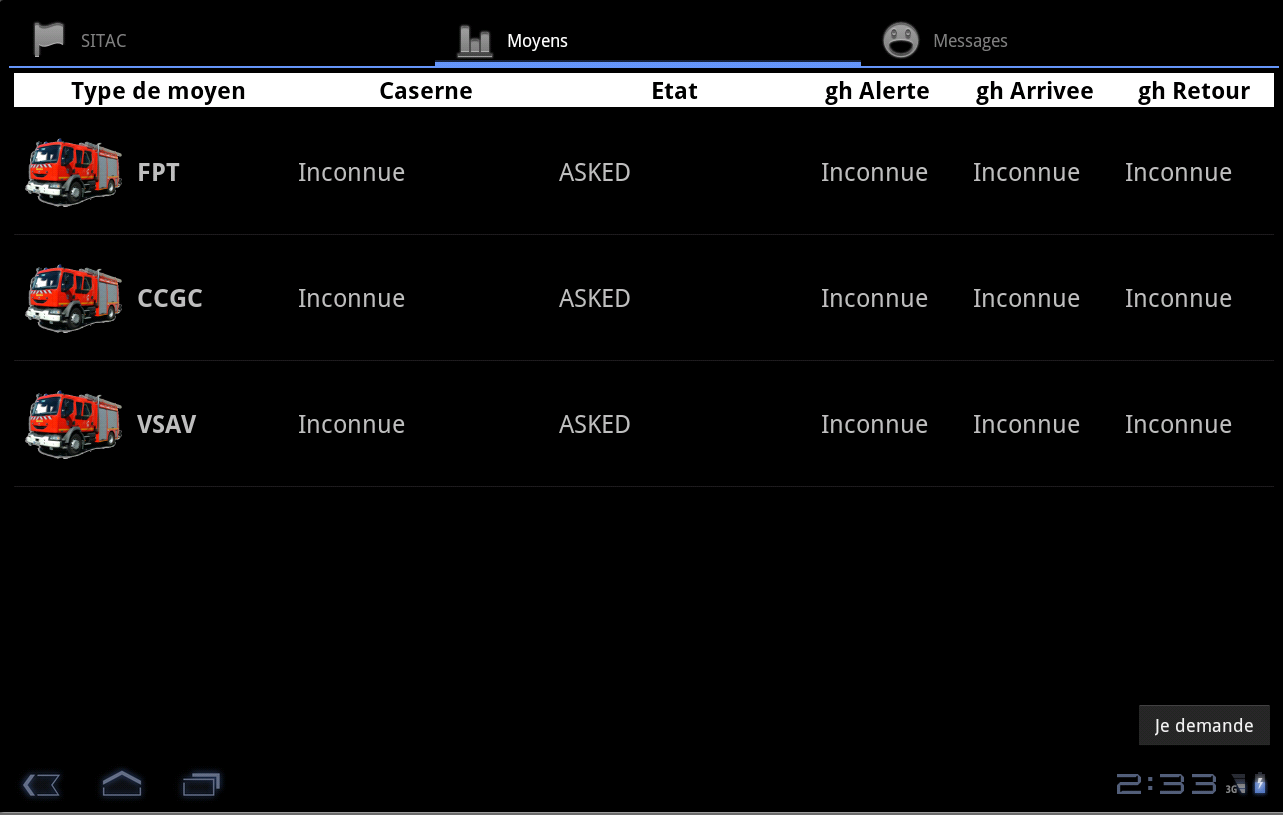
\includegraphics[width=470pt]{Manueldutilisation-fig002.png}
\caption{Tableau des moyens}
\end{center}
\end{figure}

\newpage
\subsubsection{Onglet Messages}

Cet onglet permet d’envoyer des messages au CODIS, ou de consulter l’historique des messages envoyés tout au long de l’intervention en cours.

\vspace{1.2in}

\begin{figure}[h!]
\begin{center}
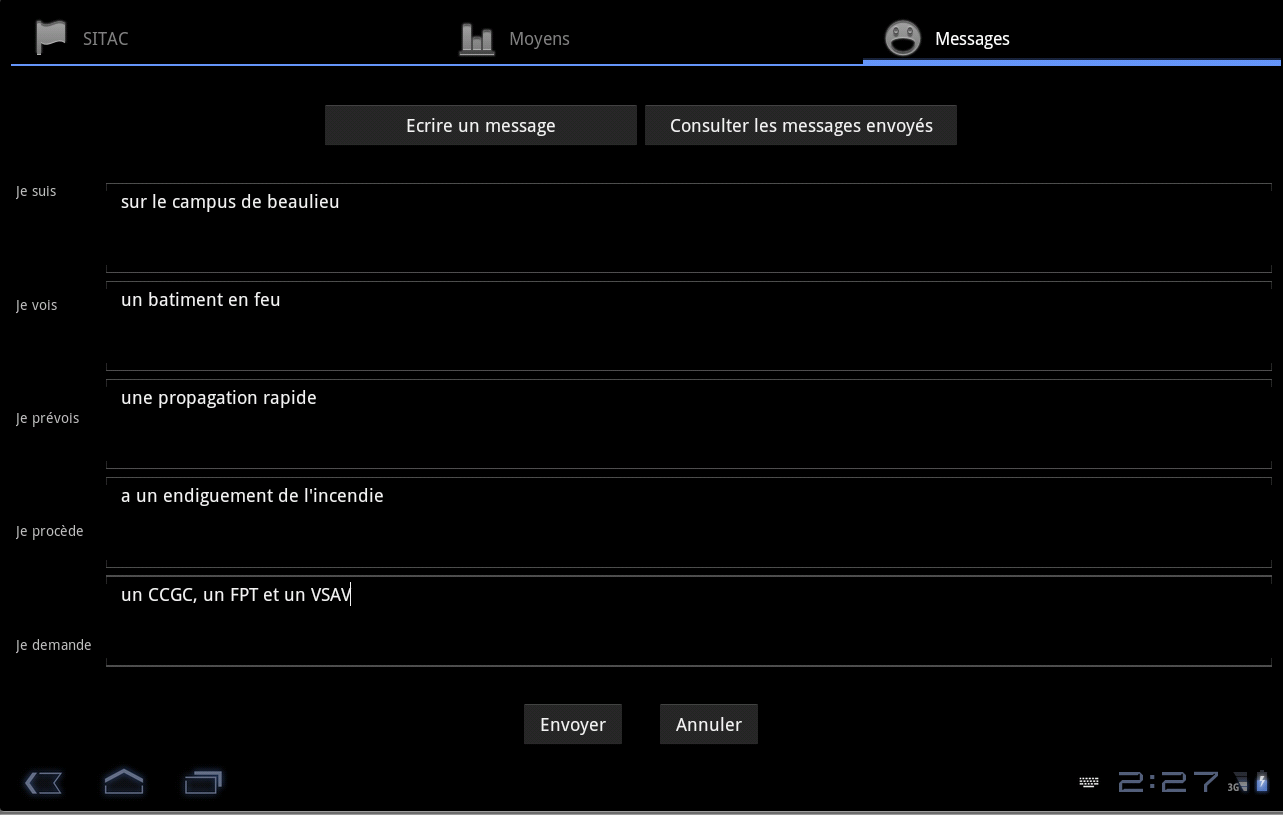
\includegraphics[width=450pt]{Manueldutilisation-fig003.png}
\caption{Vue message d'ambiance}
\end{center}
\end{figure}

\begin{figure}[h!]
\begin{center}
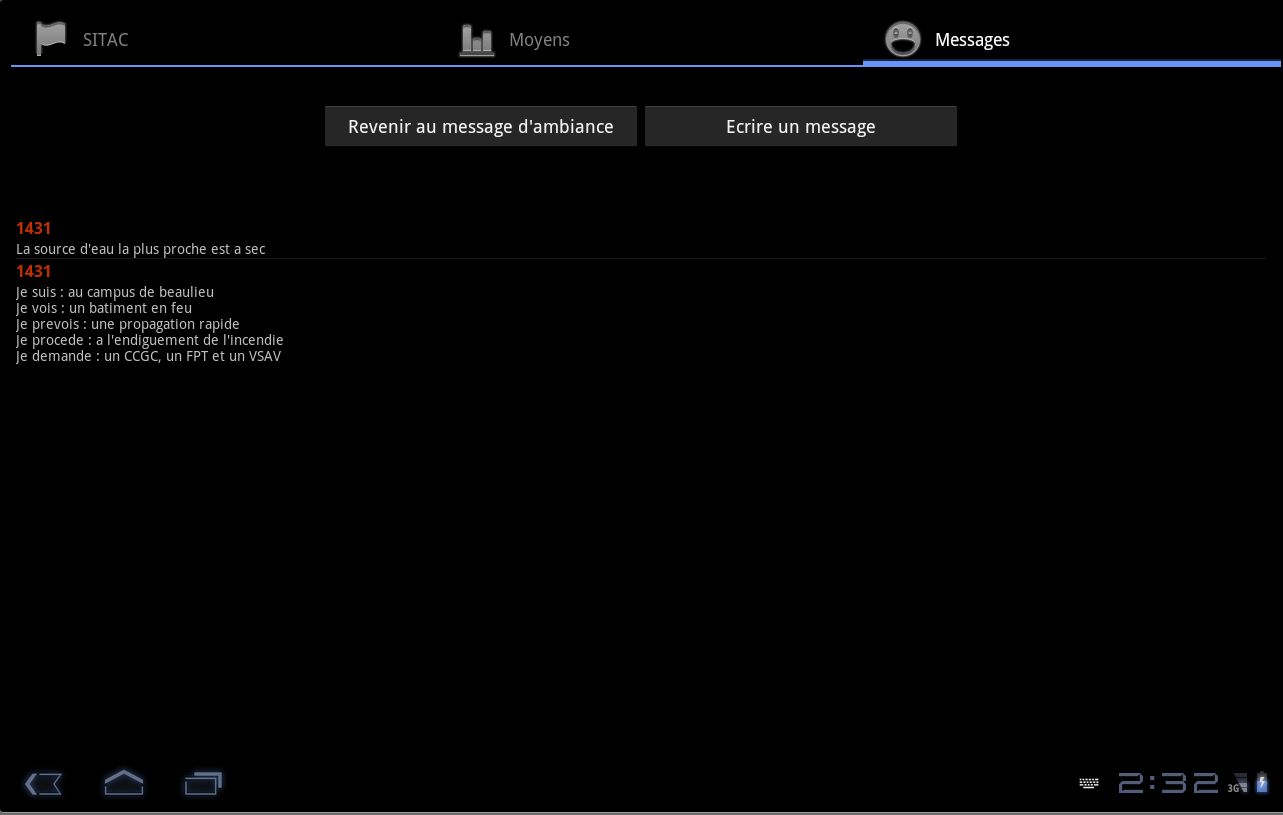
\includegraphics[width=450pt]{Manueldutilisation-fig004.png}
\caption{Historique des messages envoyés}
\end{center}
\end{figure}

\newpage
\subsection{Manipuler la SITAC}


\subsubsection{Zoom}

Grâce à la géolocalisation, la carte se charge automatiquement en fonction de votre position.

Vous pouvez zoomer ou dézoomer celle-ci en appuyant sur les boutons zoom/dézoom situés en bas de l’onglet.

\subsubsection{Placer des pictogrammes}

Pour ajouter des éléments à la carte, déroulez le menu de gauche, les outils y sont classés par catégorie. Sélectionnez une catégorie puis l’élément voulu et placez-le sur la carte à l’endroit désiré grâce à un appui long.


\subsubsection{Délimiter une zone sur la carte}

Choisir l’outil “ligne”, puis le placer sur la carte de manière à encercler la zone, tout en s’assurant que les extrémités des lignes soient en contact.


\subsubsection{Demander un moyen depuis la SITAC}

Sélectionnez le véhicule voulu dans le menu de gauche, et positionnez-le sur la carte à l’endroit ou celui-ci devra stationner à son arrivée sur les lieux du sinistre. Cette action déclenchera systématiquement la demande de ce véhicule auprès du centre de secours le plus proche.

Pour annuler une demande de moyen, appuyez quelques secondes sur le véhicule que vous venez de rajouter sur la carte puis cliquez sur la croix qui apparaît.


\subsection{Faire une demande de moyen}

Il est possible de faire une demande de moyen via l’onglet moyen ou en plaçant directement un véhicule sur la SITAC.

Depuis l’onglet moyen, cliquez sur le bouton “Je demande” situé en bas à droite de l’écran, un menu pop-up apparaîtra. Sélectionnez ensuite la catégorie du véhicule voulu, puis dans la liste de véhicules sélectionnez un véhicule. Une demande de ce moyen sera immédiatement transmise.

Tout véhicule demandé se retrouvera dans le tableau des véhicules de l’onglet moyen ainsi que leur état (demandé, arrivé, rentré).


\subsection{Gestion des moyens }

La gestion des moyens se fait depuis l’onglet “Moyens”. Vous pouvez a tout moment consulter les véhicules impliqués dans l’intervention, ainsi que toutes les informations les concernant.

La vue d'accueil se présente sous la forme d’un tableau regroupant les détails concernant les moyens engagés c’est à dire le type du moyen, sa provenance, son état (demande, arrivé, rentré), et les groupes horaires d’alerte, d’arrivée et de retour.

Pour effectuer des modifications sur l’un des véhicules présent dans le tableau, faire un appui long sur celui-ci et éditer les informations choisies.

\subsection{Envoyer/Consulter des messages}

Dans l’onglet message, il est possible d’envoyer des messages, ou de consulter un historique des messages envoyés.

Concernant l’envoi, il existe deux types de messages : message d’ambiance et message standard.

\begin{itemize}
\item Pour un message d’ambiance : complétez les champs “je suis / je vois / je prévois / je procède / je demande”, puis appuyez sur le bouton envoyer.
\item Pour un message standard : tapez le message voulu dans la zone de texte puis appuyez sur le bouton envoyer.
\end{itemize}

Vous pouvez annuler votre saisie à l’aide du bouton “Annuler” qui videra tous les champs de saisie.

Concernant la consultation de l’historique des messages envoyés, il suffit d’appuyer sur le bouton “consulter les messages envoyés” et s’affiche alors à l’écran la liste de tous les messages que vous avez envoyé depuis le début de l’intervention, le plus récent en tête de liste.

Pour naviguer entre les différentes sous-catégories de l’onglet message, il vous suffit d’utiliser les boutons situés en haut de page, qui vous permettront de passer du message standard aux messages d’ambiance ou aux messages envoyés.  Ces boutons sont toujours présents en haut de page sur les différentes vues. 

\end{document}
